\documentclass[conference]{IEEEtran}
\usepackage[utf8]{inputenc}
\usepackage[T1]{fontenc}
\usepackage{graphicx}
\usepackage{booktabs}
\usepackage{amsmath}
\graphicspath{{../figures/}}

\title{Replicating TinyCD on LEVIR-CD: A Frozen-Checkpoint Comparison with BIT and ChangeFormer V6}
\author{\IEEEauthorblockN{Shresth Keshari}
\IEEEauthorblockA{IIT Bombay}}

\begin{document}
\maketitle

\begin{abstract}
We replicate TinyCD, a lightweight Siamese U-Net for building change detection, by running its released LEVIR-CD checkpoint together with BIT and ChangeFormer V6 under one frozen-inference protocol: all 2,048 LEVIR-CD test pairs, threshold 0.5, no retraining or test-set tuning. TinyCD reaches 91.07 F1 (95\% bootstrap CI 90.63--91.45) with 0.285 M parameters and 1.46 GFLOPs. Its paired F1 margin is +1.12 over BIT and +0.67 over ChangeFormer V6. The published one-point margin therefore holds against BIT but not against ChangeFormer V6 on F1, although the IoU margin over ChangeFormer V6 is +1.11. BIT measures 89.94 F1 against 89.31 published, and we could not explain the gap. Zeroing the full-resolution attention mask drops F1 to 0.3, and all three models return no detections on a 30 m Landsat pair. The evidence supports claims about LEVIR-CD only.
\end{abstract}

\section{Introduction}
Change detection compares two co-registered images of the same place taken at different times and marks the pixels where a relevant change occurred. Here the relevant change is a building built or demolished. Changed pixels are rare: 5.09\% of LEVIR-CD test pixels, so overall accuracy is near 99\% even for weak models, and we report the change-class precision, recall, F1 and IoU instead.

TinyCD~\cite{codegoni2023tinycd} argues that a model with about 0.3 M parameters can match or beat much larger change detectors on LEVIR-CD. Its headline claim is a margin of at least one point on F1 and IoU over the strongest comparators. We test that claim by re-running the released checkpoints under a single protocol, and we report what holds and what does not.

\section{Related Work}
LEVIR-CD~\cite{chen2020levircd} is a building change dataset of Google Earth image pairs, released with a spatial-temporal attention baseline; all three models here are evaluated on its test split. BIT~\cite{chen2021bit} encodes each image pair as a small set of semantic tokens and models context with a transformer. ChangeFormer~\cite{bandara2022changeformer} is a Siamese hierarchical transformer with a lightweight MLP decoder. TinyCD instead keeps a convolutional Siamese U-Net on shared EfficientNet-B4 features~\cite{tan2019efficientnet}, fuses the two branches with a mixing block, and adds attention-mask skips.

\section{Method and Setup}
\textbf{Models.} TinyCD uses the authors' released LEVIR-CD weights, loaded with \texttt{strict=True} into our re-implementation. BIT uses the official code at a pinned commit with the \texttt{base\_transformer\_pos\_s4\_dd8\_dedim8} weights. ChangeFormer V6 uses the official release v0.1.0 with embedding dimension 256. Each checkpoint's SHA-256 was verified.

\textbf{Data.} The LEVIR-CD256 test split: 2,048 pairs of 256$\times$256 pixels at 0.5 m per pixel.

\textbf{Metrics.} Predictions are thresholded at 0.5. Precision, recall, F1 and IoU are computed for the change class from pixel counts pooled over the test set. Object recall uses 8-connected components of the ground-truth mask; a component counts as detected when at least 50\% of its pixels are predicted as change.

\textbf{Uncertainty.} We resample the 2,048 test pairs with replacement 2,000 times (seed 0), re-sum the confusion matrix, and take the 2.5th and 97.5th percentiles. Paired differences use the same resamples.

\textbf{Efficiency.} Parameters are counted both stored and used in the forward pass; GFLOPs come from fvcore. Latency is the median of 100 GPU runs and 20 CPU runs (8 threads) at batch 1, on an RTX 3050 6 GB laptop GPU.

\section{Results}
\begin{table}[t]
\centering
\caption{LEVIR-CD test, 2,048 pairs, threshold 0.5. Paper F1 is from Codegoni et al.'s LEVIR-CD comparison table. CI is the 95\% bootstrap interval for F1. Values in \%.}
\label{tab:bench}
\small
\resizebox{\columnwidth}{!}{%
\begin{tabular}{lccccc}
\toprule
Model & Paper F1 & F1 & 95\% CI & IoU & Prec./Rec. \\
\midrule
TinyCD & 91.05 & 91.07 & [90.63, 91.45] & 83.60 & 92.66 / 89.53 \\
BIT & 89.31 & 89.94 & [89.35, 90.53] & 81.72 & 90.33 / 89.56 \\
ChangeFormer V6 & 90.40 & 90.40 & [89.82, 90.93] & 82.48 & 92.06 / 88.80 \\
\bottomrule
\end{tabular}%
}
\end{table}

\textbf{Paired margins.} TinyCD minus comparator, F1: +1.12 vs BIT (95\% CI [0.69, 1.57]) and +0.67 vs ChangeFormer V6 (CI [0.29, 1.00]). Both intervals exclude zero. The IoU margin over ChangeFormer V6 is +1.11.

\begin{figure}[t]
\centering
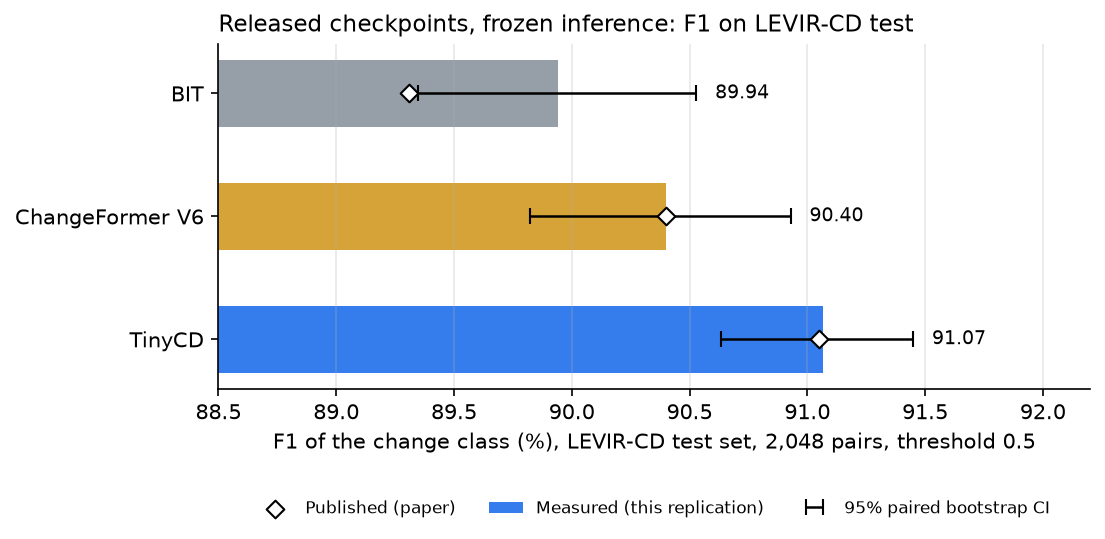
\includegraphics[width=\columnwidth]{01_benchmark_f1.png}
\caption{F1 of the change class on LEVIR-CD test: measured (bars and CIs) against published values (diamonds).}
\label{fig:f1}
\end{figure}

\begin{table}[t]
\centering
\caption{Object recall (\%) by ground-truth size (8-connected components, 8,673 objects), and cost of each model.}
\label{tab:obj}
\small
\begin{tabular}{lccc}
\toprule
 & TinyCD & BIT & ChangeFormer V6 \\
\midrule
$<$25 m$^2$ (n=825) & 32.2 & 31.4 & 35.2 \\
25--100 m$^2$ (n=1282) & 82.9 & 81.1 & 81.1 \\
100--400 m$^2$ (n=6058) & 97.6 & 97.2 & 97.0 \\
$>$400 m$^2$ (n=508) & 96.3 & 94.9 & 95.3 \\
All objects & 89.2 & 88.4 & 88.7 \\
\midrule
Params used (M) & 0.285 & 3.04 & 41.03 \\
GFLOPs & 1.46 & 8.76 & 138.8 \\
GPU latency (ms) & 24.2 & 32.3 & 103.6 \\
CPU latency (ms) & 194 & 266 & 2,454 \\
\bottomrule
\end{tabular}
\end{table}

Small buildings are the weak point for all three models. Below 25 m$^2$, recall is 31--35\% for every model, with ChangeFormer V6 highest. TinyCD produces 21 false-alarm pairs out of 1,113 no-change pairs (1.9\%), against 68 for BIT (6.1\%) and 40 for ChangeFormer V6 (3.6\%). Latency figures are specific to that laptop.

\textbf{Mask probe.} Replacing one attention mask in TinyCD with ones, on the test set (an inference-time intervention, not a retrained ablation): M256 gives F1 0.30, M64 gives 82.13, M128 gives 90.12, and all three masks together give 0.26. The released network depends heavily on the full-resolution mask. No ablation weights were released, so ablation accuracy is not measured.

\textbf{Powai (exploratory).} Applying the same checkpoints to two 30 m Landsat 8 scenes of IIT Bombay (10 February 2015 and 5 February 2025) gives zero predicted changes at threshold 0.5 for all three models. Maximum probabilities are 0.0077 (TinyCD), 0.0094 (BIT) and 0.0011 (ChangeFormer V6). The models were trained on 0.5 m imagery and no reference labels exist, so this is domain transfer, not evidence of accuracy.

\section{Discussion}
The one-point claim depends on the comparator. Against BIT, TinyCD's +1.12 F1 margin is clear. Against ChangeFormer V6 the F1 margin is +0.67: statistically positive but below one point. The paper's own published numbers give +0.65 F1 against ChangeFormer V6 and +1.09 IoU, so the F1 shortfall is not an artifact of our re-run. Our ChangeFormer V6 result matches the published 90.40 F1 and 82.48 IoU.

BIT is the open discrepancy. We measure 89.94 F1 against 89.31 published, with precision 90.33 against 89.24. We have not identified the cause; it may involve the released weights or evaluation details. Because BIT is the comparator behind the +1.12 margin, the gap matters to the headline comparison.

The mask probe shows that the mechanism is concentrated. Removing the M256 attention mask collapses performance, while removing M64 or M128 costs far less. This describes the released network; it is not evidence about which design choice is best.

\section{Conclusion}
Under one frozen-inference protocol on LEVIR-CD, TinyCD matches its published F1 (91.07) with about one tenth of BIT's used parameters and one 144th of ChangeFormer V6's, and it beats BIT by 1.12 F1 and ChangeFormer V6 by 0.67. The one-point margin holds against BIT only. The BIT gap to its published value is unexplained, and the Powai result shows that the models do not transfer to 30 m imagery without retraining.

\bibliographystyle{IEEEtran}
\bibliography{references}

\end{document}
